\documentclass{sig-alternate}
\usepackage{color}
\usepackage{graphicx}
\usepackage{url}
\usepackage{balance}  % for  \balance command ON LAST PAGE  (only there!)
\usepackage{xspace}
\usepackage[T1]{fontenc}
\usepackage{times}
%\usepackage{mathptmx}    % use "times" font, including for math mode
\usepackage{txfonts}  % apparently needed to fixup the formatting of lstlistings
\usepackage{textcomp}
\usepackage[protrusion=true,expansion=true]{microtype}
\usepackage{paralist}
\usepackage{comment}

\frenchspacing

\usepackage{listings}
\lstset{
basicstyle=\ttfamily\scriptsize,       % the size of the fonts that are used for the code
numbers=left,                   % where to put the line-numbers
numberstyle=\ttfamily,      % the size of the fonts that are used for the line-numbers
%aboveskip=0pt,
%belowskip=0pt,
stepnumber=1,                   % the step between two line-numbers. If it is 1 each line will be numbered
%numbersep=10pt,                  % how far the line-numbers are from the code
breakindent=0pt,
firstnumber=1,
%backgroundcolor=\color{white},  % choose the background color. You must add \usepackage{color}
showspaces=false,               % show spaces adding particular underscores
showstringspaces=false,         % underline spaces within strings
showtabs=false,                 % show tabs within strings adding particular underscores
frame=leftline,
tabsize=2,  		% sets default tabsize to 2 spaces
captionpos=b,   		% sets the caption-position to bottom
breaklines=false,    	% sets automatic line breaking
breakatwhitespace=true,    % sets if automatic breaks should only happen at whitespace
columns=fixed,
basewidth=0.52em,
xleftmargin=6mm,
xrightmargin=-6mm,
numberblanklines=false,
language=Ruby,
morekeywords={table,scratch,channel,interface,periodic,bloom,state,bootstrap,morph,monotone,lset,lbool,lmax,lmap},
escapeinside={(*}{*)}
}

\def\lang{Bloom$^L$\xspace}

 \newcommand{\nrc}[1]{{\textcolor{magenta}{#1 -- nrc}}}
 \newcommand{\paa}[1]{{\textcolor{blue}{[[#1 -- paa]]}}}

% \newcommand{\wrm}[1]{{\textcolor{blue}{#1 -- wrm}}}
% \newcommand{\jmh}[1]{{\textcolor{red}{#1 -- jmh}}}

\newtheorem{example}{Example}

\begin{document}

\title{Logic and Lattices for Distributed Programming}

\numberofauthors{5}

\author{
\alignauthor
Neil Conway\\
       \affaddr{UC Berkeley}\\
       \email{nrc@cs.berkeley.edu}
\alignauthor
William R.\ Marczak\\
       \affaddr{UC Berkeley}\\
       \email{wrm@cs.berkeley.edu}
\alignauthor
Peter Alvaro\\
       \affaddr{UC Berkeley}\\
       \email{palvaro@cs.berkeley.edu}
\and
\alignauthor
Joseph M.\ Hellerstein\\
       \affaddr{UC Berkeley}\\
       \email{hellerstein@cs.berkeley.edu}
\alignauthor
David Maier\\
       \affaddr{Portland State University}\\
       \email{maier@cs.pdx.edu}
}

\maketitle

\begin{abstract}
  In recent years there has been interest in achieving application-level
  consistency criteria without the latency and availability costs of strongly
  consistent storage infrastructure. A standard technique
  %, found in designs such
  % as Bayou, Escrow Transactions, and CRDTs, 
  is to adopt a vocabulary of
  commutative operations; this avoids the risk of inconsistency due to message
  reordering.  A more powerful approach was recently captured by the \emph{CALM
    Theorem}, which proves that logically monotonic programs are guaranteed to
  be eventually consistent. 
  In logic languages such as Bloom, CALM analysis can automatically verify that program modules achieve consistency without coordination.

  In this paper we present \lang, an extension to Bloom that takes inspiration
  from both these traditions.  
  % Drawing on systems that use commutative
  %   operations, \lang guarantees convergence for user-defined objects by adopting
  %   the notion of extensible \emph{lattice} data types: classes with a commutative
  %   and associative merge function.  
  \lang generalizes Bloom to support lattices
  and extends the power of CALM analysis to whole programs containing arbitrary
  lattices. We show how the Bloom interpreter can be generalized to support
  efficient evaluation of lattice-based code using well-known strategies from
  logic programming.  Finally, we use \lang to develop several practical
  distributed programs, including a key-value store similar to Amazon Dynamo,
  and show how \lang encourages the safe composition of small, easy-to-analyze
  lattices into larger programs.
\end{abstract}

\section{Introduction} 
\label{sec:intro} 
Although distributed programming has become an essential and commonplace task,
it remains very challenging for most developers to write correct distributed
programs. The inherent difficulties of distributed computing---concurrency,
asynchrony, and partial failure---are exacerbated by the scale at which modern
distributed systems operate.

% remind reviewers that it's a database problem. can remove if accepted! 
Much of the discussion about distributed programming today revolves around data
management systems, and the tradeoffs between transactions and loose
consistency. Programmers using distributed transactions are relieved of
consistency concerns but often face significant performance and operational
challenges~\cite{Birman2009}. By contrast, programmers who use loosely
consistent systems can expect more predictable and low-latency performance, but
must reason explicitly about program correctness over inconsistent distributed
state.

In recent years there has been increased interest in techniques to help
programmers achieve correct program behavior without requiring strongly
consistent storage. This idea has been explored in two different frameworks,
\emph{Convergent Objects} and \emph{Monotonic Logic}.

\vspace{0.5em}\noindent
\textbf{Convergent Objects}: In this approach, a programmer writes encapsulated
object classes whose public methods guarantee certain properties regarding
message reordering and/or retry. For example, Statebox is an open-source library
that merges conflicting updates to data items in a key-value store; the user of
the library need only register commutative, idempotent merge
functions~\cite{statebox}. This approach has roots in research in
databases~\cite{Farrag1989,Garcia-Molina1983,Helland2009} and
groupware~\cite{Ellis1989,Sun1998}.  Shapiro et al.\ recently proposed a model
for these approaches called \emph{Conflict-Free Replicated Data Types} (CRDTs),
which formalizes these ideas in an algebraic framework~\cite{Shapiro2011b}.

The main problem with the CRDT approach is that its guarantees of correctness
are limited to an individual replicated data value, not to application logic in
general. For example, consider a distributed algorithmic trading service that
uses a CRDT to represent a mutable set \texttt{Portfolio}. Suppose one server
$M$ reads a local version of the set containing an element \texttt{BNNA} and
constructs an expected portfolio value $v = f(\mbox{\texttt{Portfolio}})$
derived from that version. Concurrently, \texttt{BNNA} is removed from the local
version of \texttt{Portfolio} at another server $N$. The CRDT can ensure that
$M$ and $N$ will eventually agree that \texttt{BNNA} is absent from the set, but
the application state at $M$ and $N$ may remain inconsistent unless the value
$v$ at $M$ is updated to reflect the removal of \texttt{BNNA}. Although the CRDT
maintains its own invariants, the programmer still bears the burden of ensuring
the consistency semantics of the entire program.

\vspace{0.5em} \noindent
\textbf{Monotonic Logic}: In recent work, we observed that the database theory
literature on non-monotonic logic provides a promising starting point for
reasoning about distributed consistency. Intuitively, a \emph{monotonic} program
computes more information over time---it never ``retracts'' an earlier
conclusion in the face of new information. We proposed the CALM
theorem~\cite{Hellerstein2010}, which established that all monotonic programs
are eventually consistent~\cite{Ameloot2011,dedalus-pods12-tr}. Monotonicity of
a Datalog-style program is straightforward to determine conservatively from
syntax, so the CALM theorem provides the basis for a simple analysis technique
for verifying the consistency of distributed programs~\cite{Alvaro2011}. We
realized the CALM analysis as part of Bloom, a Datalog-based DSL for distributed
programming~\cite{bloom}.

The original formulation of Bloom and CALM only validated consistency for programs that compute sets of facts that grow over time (``set monotonicity''); that is, ``growth'' is defined according to set containment. As a practical matter, this is overly conservative: several common distributed programming idioms that are monotonic do not satisfy syntactic monotonicity tests for Datalog. In particular, threshold tests over monotonic aggregate values (e.g., ``$\mathrm{max}(S) > k$'') and upward-moving mutable counters are both considered to be non-monotonic by the original CALM analysis.  As a result, the initial Bloom prototype advises the programmer to guard those constructs with strong consistency methods like Paxos~\cite{Lamport1998} or Two-Phase Commit. 

\subsection{A Hybrid Approach}
% The strengths and weaknesses of these two approaches appear complementary. CRDTs provide synchronization-free consistent objects, but cannot guarantee whole-program consistency. Bloom's CALM analysis guarantees whole-program consistency but is unable to verify a number of natural coordination-free mechanisms.
In this paper, we extend our previous work to accommodate the ideas underlying CRDTs. Instead of only allowing growth according to the set containment
partial order, we allow any user-defined partial order to be used.  
We do this by providing \emph{join semi-lattices} as a programming construct.
We give a
formal definition of this construct below, but the intuition is that the programmer provides a commutative, idempotent merge function (``least upper bound'')
that takes two input values and produces an output value that is not smaller
than either of the input values (according to the user's partial order). This
generalizes Bloom (and traditional Datalog), which assumes a fixed merge
function (set union) and partial order (set containment).
% Relate user-defined merge functions to merge functions in other contexts?
% (e.g., key-value store, COPS, Piccolo)

% Explain how lattices generalize monotonic datalog
It is attractive to incorporate join semi-lattices into logic programming,  but doing so raises challenges in language design, consistency analysis and efficient execution.  In this paper, we make the following contributions:
\begin{enumerate}
% \item
%   We present \baselang, a variant of Datalog that is defined over lattices. We
%   define a model-theoretic semantics for \baselang, and show that \baselang
%   generalizes Datalog.

\item
  We introduce \lang, an extension of Bloom that supports lattices. We detail
  the builtin lattice types provided by \lang and show how developers can
  define new lattices.
  
\item 
  We provide interfaces for consistency-preserving mappings across lattices via
  \emph{morphisms} and \emph{monotonic functions}.  This is critical for \lang
  and forms a useful extension to the CRDT framework as well.

\item 
  We generalize the CALM analysis to programs that contain both lattices and
  set-oriented collections, and show how lattices can be used to prove the
  confluence of several common distributed design patterns that were regarded as
  non-monotonic in Bloom. % XXX: revisit this

\item
  For efficient execution, we show how to extend the standard Datalog semi-naive
  evaluation scheme~\cite{Balbin1987} to support both lattices and traditional
  database relations. We also describe how an existing Datalog engine can be
  extended to support lattices with relatively minor changes.

\item
  Finally, we demonstrate the usefulness of lattices with two case studies.
  First we revisit the simple e-commerce scenario presented in Alvaro et al., in
  which clients interact with a replicated shopping cart
  service~\cite{Alvaro2011}. We show how \lang can be used to make the
  ``checkout'' operation monotonic, despite the fact that it requires
  aggregating over a distributed data set.

  Second, we use \lang to implement vector clocks and causal delivery, two
  standard building blocks for distributed programming. We show how both
  algorithms can be realized as monotonic \lang programs that are concise and
  readable.
\end{enumerate}

\section{Background}
\label{sec:background}

% XXX: should this be a distributed example?
\begin{figure}[t]
\begin{scriptsize}
\begin{lstlisting}
class ShortestPaths
  include Bud

  state do
    table :link, [:from, :to] => [:cost] (*\label{line:spaths-ddl}*)
    scratch :path, [:from, :to, :next_hop, :cost]
    scratch :min_cost, [:from, :to] => [:cost]
  end

  bloom do
    path <= link {|l| [l.from, l.to, l.to, l.cost]} (*\label{line:spaths-proj}*)
    path <= (link*path).pairs(:to => :from) do |l,p| (*\label{line:spaths-join-start}*)
      [l.from, p.to, l.to, l.cost + p.cost]
    end (*\label{line:spaths-join-end}*)

    min_cost <= path.group([:from, :to], min(:cost)) (*\label{line:spaths-group}*)
  end
end
\end{lstlisting}
\end{scriptsize}
\caption{All-pairs shortest paths in Bloom.}
\label{fig:bloom-spaths}
\end{figure}

In this section, we review the Bloom programming language and the CALM program
analysis.  We highlight a simple distributed program for which the CALM analysis
yields unsatisfactory results.

\subsection{Bloom}
\label{sec:bg-bloom}

Bloom is a Datalog-based domain-specific language (DSL) for distributed
programming~\cite{Alvaro2011,bloom}. The state of a Bloom program is represented
using \emph{collections} and computation is expressed as a bundle of declarative
\emph{statements}.  An instance of a Bloom program performs computation by
evaluating its statements over the contents of its local database. Bloom
instances communicate via asynchronous messaging, as described further below.

An instance of a Bloom program proceeds through a series of \emph{timesteps},
each containing three phases.\footnote{There is a precise declarative semantics
  for Bloom~\cite{dedalus}, but we describe the language operationally for the
  sake of exposition.} In the first phase, inbound events (e.g., network
messages) are received and represented as facts in collections. In the second
phase, the program's statements are evaluated over local state to compute all
the additional facts that can be derived from the current collection
contents. In some cases (described below), a derived fact is intended to achieve
a ``side effect,'' such as modifying local state or sending a network message.
These effects are deferred during the second phase of the timestep; the third
phase is devoted to carrying them out.

The initial implementation of Bloom, called \emph{Bud}, allows Bloom logic to be
embedded inside a Ruby program. Figure~\ref{fig:bloom-spaths} shows a Bloom
program represented as an annotated Ruby class. A small amount of imperative
Ruby code is needed to instantiate the Bloom program and begin executing it;
more details are available on the Bloom language website~\cite{bloom}.

\subsubsection{Data model}
\begin{table}[t]
\begin{tabular}{|l|p{2.32in}|}
\hline
\textbf{Name} & \textbf{Behavior }\\
\hline
\texttt{table} & Persistent storage.\\
\texttt{scratch} & Transient storage.\\
\texttt{channel} & Asynchronous communication. A fact derived into a \texttt{channel} appears in the
database of a remote Bloom instance at a non-deterministic future time.\\
\texttt{periodic} & Interface to the system clock.\\
\texttt{interface} & Interface point between software modules.\\
\hline
\end{tabular}
\caption{Bloom collection types.}
\label{tbl:bloom-collections}
\end{table}

The Bloom data model is based on \emph{collections}.  A collection is an
unordered set of \emph{facts}, akin to a relation in Datalog. The Bud prototype
adopts the Ruby type system rather than inventing its own; hence, a fact in Bud
is just an array of Ruby objects. Each collection has a \emph{schema}, which
declares the structure (column names) of the facts in the collection. A subset
of the columns in a collection form its \emph{key}: as in the relational model,
the key columns functionally determine the remaining columns. The collections
used by a Bloom program are declared in a \texttt{state} block. For example,
line~\ref{line:spaths-ddl} of Figure~\ref{fig:bloom-spaths} declares a
collection named \texttt{link} with three columns, two of which form the
collection's key. Ruby is a dynamically typed language, so keys and values in
Bud can hold arbitrary Ruby objects.

Bloom provides five collection types to represent different kinds of state
(Table~\ref{tbl:bloom-collections}). A \texttt{table} stores persistent data: if
a fact appears in a table, it remains in the table in future timesteps (unless it
is explicitly removed). A \texttt{scratch} contains transient data---the content
of scratch collections is emptied at the start of each timestep. Scratches are
akin to SQL views: they are often useful as a way to name intermediate results
or as a ``macro'' construct to enable code reuse. The \texttt{channel}
collection type enables communication between Bloom instances. The schema of a
channel has a distinguished \emph{location specifier} column (prefixed with
``\texttt{@}''); when a fact is derived for a channel collection, it appears in
the database of the Bloom instance at the address given by the location
specifier. The \texttt{periodic} and \texttt{interface} collection types do not
arise in our discussion in this paper; the interested reader is referred to the
Bloom website~\cite{bloom}.

\subsubsection{Statements}
\begin{table}
\begin{tabular}{|c|l|p{1.85in}|}
\hline
\textbf{Op} & \textbf{Name} & \textbf{Meaning} \\
\hline
\verb|<=| & \emph{merge} & lhs includes the content of rhs in the
current timestep \\
\hline
\verb|<+| & \emph{deferred merge} & lhs will include the content of rhs in the
next timestep \\
\hline
\verb|<-| & \emph{deferred delete} & lhs will not include the content of rhs
in the next timestep \\
\hline
\verb|<~| & \emph{async merge} & (remote) lhs will include the content of the
rhs at some non-deterministic future timestep\\
\hline
\end{tabular}
\caption{Bloom operators.}
\label{tbl:bloom-ops}
\end{table}

Each Bloom statement has one or more input collections and a single output
collection.  A statement takes the form: \\ \noindent
\mbox{\hspace{0.25in}\emph{$<$collection-identifier$>$ $<$op$>$
    $<$collection-expression$>$}}\\ \noindent
The left-hand side (lhs) is the name of the output collection and the right-hand
side (rhs) is an expression that produces a collection.  A statement defines how
the contents of the input collections should be transformed before being
included (via set union) in the output collection. Bloom allows the usual
relational operators to be used on the rhs (selection, projection, join,
grouping, aggregation, and negation), although it adopts a syntax intended to be
more familiar to imperative programmers. In Figure~\ref{fig:bloom-spaths},
line~\ref{line:spaths-proj} demonstrates projection,
lines~\ref{line:spaths-join-start}--\ref{line:spaths-join-end} perform a join
between \texttt{link} and \texttt{path} using the join predicate
\verb+link.to = path.from+ followed by a projection to four attributes, and
line~\ref{line:spaths-group} demonstrates grouping and aggregation. Bloom
statements appear in one or more \texttt{bloom} blocks. A Bloom program can also
include a \texttt{bootstrap} block, which contains statements that are evaluated
only once when a Bloom instance starts executing. \texttt{bootstrap} blocks are
typically used for initialization or configuration data.

Bloom provides several operators that determine \emph{when} the rhs will be
merged into the lhs (Table~\ref{tbl:bloom-ops}). The \verb|<=| operator performs
standard logical deduction: that is, the lhs and rhs are true at the same
timestep. The \verb|<+| and \verb|<-| operators indicate that facts will be
added or removed, respectively, from the lhs collection at the beginning of the
\emph{next} timestep. The \verb+<~+ operator specifies that the rhs will be merged into
the lhs collection at some non-deterministic future time. The lhs of a statement
that uses \verb+<~+ must be a channel; the \verb+<~+ operator captures
asynchronous messaging.

% XXX: does this need to be said?
Bloom allows recursion---i.e., the rhs of a statement can reference the lhs
collection, either directly or indirectly. As in Datalog, certain constraints
must be adopted to ensure that programs with recursive statements have a
sensible interpretation. For deductive statements (\verb+<=+ operator), we
require that programs be \emph{syntactically stratified}~\cite{Apt1988}: cycles
through negation or aggregation are not allowed (unless they contain a deferred
or asynchronous operator)~\cite{dedalus}.

\subsection{CALM analysis}
\label{sec:bg-calm}

Work on deductive databases has long drawn a distinction between
\emph{monotonic} and \emph{non-monotonic} logic programs. Intuitively, a
monotonic program only computes more information over time---it will never
``retract'' a previous conclusion in the face of new evidence.  In Bloom (and
Datalog), a simple conservative test for monotonicity is based on program
syntax: selection, projection, and join are monotonic, while aggregation and
negation are not.

The CALM theorem connects the theory of monotonic logic with the practical
problem of distributed consistency~\cite{Alvaro2011,Hellerstein2010}.  All
monotonic programs are ``eventually consistent'' or \emph{confluent}: for any
given input, all program executions result in the same final state regardless of
network non-determinism~\cite{Ameloot2011,dedalus-confluence}.  Hence, monotonic
logic is a useful building block for loosely consistent distributed programming.

According to the CALM theorem, distributed inconsistency may only occur at
\emph{points of order}: program locations where the output of an asynchronously
derived value is consumed by a non-monotonic operator.  This is because
asynchronous messaging results in non-deterministic arrival order, and
non-monotonic operators may be produce different conclusions when evaluated over
different subsets of their inputs.  For example, consider a Bloom program in
which collections $A$ and $B$ are fed by asynchronous channels and the program
sends a message whenever an element of $A$ arrives that is not in $B$. This
program is non-monotonic and exhibits non-confluent behavior: the messages sent
by the program will depend on the order in which the elements of $A$ and $B$
arrive.

We have implemented a conservative static program analysis in Bloom that follows
directly from the CALM theorem.  Programs that are free from non-monotonic
constructs are ``blessed'' as confluent: producing the same output on different
runs or converging to the same state on multiple distributed replicas.
Otherwise, programs are flagged as potentially inconsistent.  To achieve
consistency, the programmer either needs to rewrite their program to avoid the
use of non-monotonicity or introduce a coordination protocol to ensure that a
consistent ordering is agreed upon. Coordination protocols incur additional
latency and reduce availability in the event of network partitions, so in this
paper we focus on coordination-free designs---that is, monotonic programs.

\subsubsection{Limitations of set monotonicity}
The original formulation of the CALM theorem considered only programs that
compute more facts over time---that is, programs whose output \emph{sets} grow
monotonically. Many distributed protocols make progress over time, but their
notion of ``progress'' is often difficult to represent as a growing set of
facts. For example, consider the Bloom program in
Figure~\ref{fig:bloom-nm-quorum}. This program receives votes from a client
program (not shown) via the \texttt{vote\_chn} channel. Once at least
\texttt{QUORUM\_SIZE} votes have been received, a message is sent to a remote
node to indicate that quorum has been reached
(line~\ref{line:bloom-quorum-msg}). This program resembles a ``quorum vote''
subroutine that might be used by an implementation of Paxos~\cite{Lamport1998}
or quorum replication~\cite{Gifford1979}.

It is easy to see that this program makes progress in a semantically monotonic
fashion: the set of received votes grows and the size of the \texttt{votes}
collection can only increase, so once a quorum has been reached it will never be
retracted. Unfortunately, the current CALM analysis would regard this program as
non-monotonic because it contains aggregation (the grouping operation on
line~\ref{line:bloom-nm-quorum}).

To solve this problem, we need to introduce a notion of program values that
``grow'' according to a partial order other than set containment. We do this by
extending Bloom to operate over arbitrary lattices, rather than just the
set lattice.

%  We present a
% complete language in the following section, but the intuition can be observed in
% Figure~\ref{fig:lattice-quorum}. Votes are accumulated into a set lattice
% (line~\ref{line:quorum-set-accum}), but the size of the set is represented as an
% \texttt{lmax} lattice (line~\ref{line:quorum-lmax}): that is, a number that
% never decreases. Hence, a threshold test ``$\ge k$'' on an \texttt{lmax} lattice
% is monotonic map onto the boolean lattice: that is, the \texttt{quorum\_done}
% predicate goes from false to true (and then remains true).

\begin{figure}[t]
\begin{scriptsize}
\begin{lstlisting}
QUORUM_SIZE = 5
RESULT_ADDR = "example.org"

class QuorumVote
  include Bud

  state do
    channel :vote_chn, [:@addr, :voter_id]
    channel :result_chn, [:@addr]
    table   :votes, [:voter_id]
    scratch :cnt, [] => [:cnt]
  end

  bloom do
    votes      <= vote_chn {|v| [v.voter_id]}
    cnt        <= votes.group(nil, count(:voter_id)) (*\label{line:bloom-nm-quorum}*)
    result_chn <~ cnt {|c| [RESULT_ADDR] if c >= QUORUM_SIZE} (*\label{line:bloom-quorum-msg}*)
  end
end
\end{lstlisting}
\end{scriptsize}
\caption{A non-monotonic Bloom program that waits for a quorum of votes to be received.}
\label{fig:bloom-nm-quorum}
\end{figure}

\section{Adding Lattices to Bloom}
\label{sec:lang}

In this section, we introduce \lang, an extension to Bloom that allows monotonic
programs to be written using arbitrary lattices. We begin by reviewing the
algebraic properties of lattices, monotone functions, and morphisms. We then
introduce the basic concepts of \lang and detail the builtin lattices provided
by the language. We also show how users can define their own lattice types using
a simple API.

% is this the right place for this?
When designing \lang, we decided to extend Bloom to include support for lattices
rather than building a new language from scratch. Hence, \lang is backward
compatible with Bloom and was implemented with relatively minor changes to the
Bud runtime. This design decision also required that we consider how code
written using lattices should interoperate with traditional Bloom relations; we
added several \lang features to ease this interoperability, which we describe in
Section~\ref{sec:bloom-interop}.

\subsection{Definitions}
\label{sec:lattice-defn}
A \emph{bounded join semilattice} is a triple $\langle S, \lor, \bot\rangle$,
where $S$ is a poset, $\lor$ is a binary operator (called ``join'' or ``least
upper bound''), and $\bot \in S$. $\lor$ is associative, commutative, and
idempotent. For all $x, y \in S$, $x \lor y = z$, where $x \leq_S z, y \leq_S
z$, and there is no $z' \ne z \in S$ such that $z' \leq_S z$ (where $\leq_S$ is
the partial order of poset $S$). Note that although the underlying set only has
a partial order, the least upper bound is defined for all elements $x,y \in
S$. The distinguished element $\bot$ is the smallest element in $S$; this
implies that $x \lor \bot = x$ for all $x \in S$. For brevity, we use the term
``lattice'' to mean ``bounded join semilattice'' in the rest of this paper.

% XXX: note that algebraic properties that must be satisfied by morphisms and
% monotone functions
A \emph{monotone function} from poset $S$ to poset $T$ is a function $f: S \to
T$ such that $\forall a,b \in S: a \leq_S b \Rightarrow f(a) \leq_T f(b)$. That
is, $f$ maps elements of $S$ to elements of $T$ in a manner that is consistent
with the partial orders of both posets.

% XXX: mention that morphisms must be distributive with respect to the lub of
% their domain, whereas monotone functions don't need to be?
A \emph{morphism} from lattice $\langle X, \lor_X, \bot_X\rangle$ to lattice
$\langle Y, \lor_Y, \bot_Y\rangle$ is a function $g: X \to Y$ such that,
$\forall a,b \in X: g(a \lor_X b) = g(a) \lor_Y g(b)$. That is, $g$ allows
elements of $X$ to be converted into elements of $Y$ in a way that preserves the
lattice properties.  Note that morphisms are monotone functions but the converse
is not true in general.

\subsection{Language concepts}
\begin{figure}[t]
\begin{scriptsize}
\begin{lstlisting}
QUORUM_SIZE = 5
RESULT_ADDR = "example.org"

class QuorumVoteL
  include Bud

  state do
    channel :vote_chn, [:@addr, :voter_id]
    channel :result_chn, [:@addr]
    lset    :votes (*\label{line:quorum-lset-decl}*)
    lmax    :cnt
    lbool   :quorum_done
  end

  bloom do
    votes       <= vote_chn {|v| v.voter_id} (*\label{line:quorum-set-accum}*)
    cnt         <= votes.size (*\label{line:quorum-size}*)
    quorum_done <= cnt.gt_eq(QUORUM_SIZE) (*\label{line:quorum-threshold}*)
    result_chn  <~ quorum_done.when_true { [RESULT_ADDR] }
  end
end
\end{lstlisting}
\end{scriptsize}
\caption{A monotonic \lang program that waits for a quorum of votes to be received.}
\label{fig:lattice-quorum}
\end{figure}

\lang allows both lattices and collections to be used to represent state. A
lattice is analogous to a collection type in Bloom, while a lattice element
corresponds to a collection with a particular value. For example, the
\texttt{lset} lattice is similar to the \texttt{table} collection type provided
by Bloom; an element of the \texttt{lset} lattice is a particular set. In the
terminology of object-oriented programming, a lattice is a class that obeys a
certain interface and an element of a lattice is an instance of that
class. Figure~\ref{fig:lattice-quorum} contains an example \lang program.

As with collections, the lattices used by a \lang program are declared in a
\texttt{state} block. More precisely, a state block declaration introduces an
identifier that is associated with a lattice element; over time, the binding
between identifiers and lattice elements is updated to reflect state changes in
the program. For example, line~\ref{line:quorum-lset-decl} of
Figure~\ref{fig:lattice-quorum} declares an identifier \texttt{votes} that is
mapped to an element of the \texttt{lset} lattice. As more votes are received,
the lattice element associated with the \texttt{votes} identifier changes (it
moves ``upward'' in the \texttt{lset} lattice). When a lattice identifier is
declared, it is initially bound to the value $\bot$, the ``least element'' in
the lattice's underlying poset. For example, an \texttt{lset} lattice initially
contains the empty set.

\subsubsection{Statements in \lang}
Statements take the same form in both Bloom and \lang: \\ \noindent
\mbox{\hspace{0.25in}\emph{$<$identifier$>$ $<$op$>$
    $<$expression$>$}}\\ \noindent
The identifier on the lhs can refer to either a set-oriented collection or a
lattice. The expression on the rhs can contain both traditional relational
operators (applied to Bloom collections) and methods invoked on lattices.
Lattice methods are similar to methods in an object-oriented language and are
invoked using the standard method invocation syntax. For example,
line~\ref{line:quorum-size} of Figure~\ref{fig:lattice-quorum} invokes the
\texttt{size} method on an element of the \texttt{lset} lattice.

If the lhs of a statement is a lattice, the statement's operator must be either
\verb|<=| or \verb|<+| (instantaneous or deferred deduction, respectively). The
meaning of this operator is that, at either the current or the following
timestep, the lhs identifier will take on the result of applying the lattice's
least upper bound to the lhs and rhs lattice elements. The intuition remains the
same as in Bloom: the rhs value is ``merged into'' the lhs lattice, except that
the semantics of the merge operation are defined by the lattice's least upper
bound operator. We also require that the lhs and rhs refer to a lattice of the
same type.

\lang does not currently support a notion of deletion (\verb|<-| operator) for
lattices. Lattices do not directly support asynchronous communication (via the
\verb|<~| operator) but lattice elements can be embedded into tuples that appear
channels (Section~\ref{sec:bloom-interop}).

\subsubsection{Lattice methods}
\lang statements compute values over lattices by invoking methods on lattice
elements. Just as a subset of the relational operators (selection, projection,
and join) are monotonic, some lattice methods are monotone functions as defined
in Section~\ref{sec:lattice-defn}. The input to a monotone lattice method is the
receiver of the method invocation. A monotone method guarantees that, if the
input to the method grows (according to the input's lattice type), the value
returned by the function will grow (according to the result value's lattice
type).

A lattice method's signature indicates its monotonicity properties. More
precisely, \lang distinguishes between methods that are monotone and a subset of
monotone methods that are \emph{morphisms}. The properties that a morphism must
satisfy are given formally in Section~\ref{sec:lattice-defn}, but the intuition
is that morphism on lattice $t$ can be distributed over $t$'s least upper bound
operator. This allows a variant of semi-naive evaluation for lattice programs,
as we detail further in Section~\ref{sec:lattice-eval-strat}.

Lattices can also define non-monotonic methods. Invoking a non-monotonic lattice
method in a statement is analogous to using a non-monotonic relational operator
in Bloom: the Bud interpreter stratifies the program to ensure that the input
value is computed exactly before allowing the non-monotonic operator to be
invoked. This implies that statements that cycles through non-monotonic lattice
method invocations will be rejected. As a design principle, developers are
encouraged to minimize the use of non-monotonic lattice methods in \lang: as the
CALM analysis suggests, non-monotonic reasoning may need to be augmented with
coordination to ensure consistent results.

Every lattice defines a non-monotonic method \texttt{reveal} which returns a
representation of the lattice element as a plain Ruby value. For example, the
\texttt{reveal} method on a \texttt{lset} lattice returns a Ruby array
containing the elements in the set. This is non-monotonic because once the
underlying Ruby value has been extracted from the set, \lang cannot ensure that
subsequent code uses the value in a monotonic fashion.

\subsection{Builtin lattices}
\label{sec:lattice-builtins}

\begin{table*}[t]
\begin{tabular}{|l|l|l|l|l|l|}
\hline
\textbf{Name} & \textbf{Description} & $\bot$ & \textbf{Merge$(a,b)$} & \textbf{Morphisms} &
\textbf{Monotone functions}\\
\hline
\texttt{lbool} & Boolean lattice (false $\to$ true) & \texttt{false} & $a \lor b$ & \texttt{when\_true} & \\
\texttt{lmax} & Max over an ordered domain & $-\infty$ & $max(a, b)$ &\texttt{gt},
\texttt{gt\_eq}, \texttt{+}, \texttt{-} & \\
\texttt{lmin} & Min over an ordered domain & $\infty$ & $min(a, b)$ &\texttt{lt}, \texttt{lt\_eq},
\texttt{+}, \texttt{-} & \\
\texttt{lset} & Set of values & $\emptyset$ & $a \cup b$ & \texttt{intersect}, \texttt{product},
\texttt{project}, \texttt{contains?} & \texttt{size} \\
\texttt{lpset} & Set of non-negative numbers & $\emptyset$ & $a \cup b$ &
\texttt{intersect}, \texttt{product}, \texttt{project}, \texttt{contains?} & \texttt{size}, \texttt{sum} \\
\texttt{lbag} & Multiset of values && $a \cup b$ & \texttt{intersect},
\texttt{project}, \texttt{mult}, \texttt{contains?}, \texttt{+} & \texttt{size}\\
\texttt{lmap} & Map from key to lattice values & & &
\texttt{intersect}, \texttt{project}, \texttt{at}, \texttt{key?} & \texttt{size}\\
\hline
\end{tabular}
\caption{Builtin lattices in \lang.}
\label{tbl:builtin-lattices}
\end{table*}

Table~\ref{tbl:builtin-lattices} lists the builtin lattices provided by
\lang. Many common distributed protocols can be expressed using these lattices
(e.g., the causal delivery protocol described in Section~\ref{sec:causal}).

Note that \emph{size} is a monotone function provided by several lattices, but
it is not a morphism. This is because \texttt{size} cannot be distributed over
the merge functions of those lattices. For example, \ldots

\subsection{User-defined lattices}
% XXX: note that we omit some methods from lset
\begin{figure}[t]
\begin{scriptsize}
\begin{lstlisting}[deletekeywords={lset}]
class Bud::SetLattice < Bud::Lattice
  wrapper_name :lset (*\label{line:lset-wrapper-name}*)

  def initialize(x=[])
    # Reject invalid input (elided)
    @v = x.uniq # Remove duplicates from input
  end

  def merge(i)
    self.class.new(@v | i.reveal)
  end

  morph :intersect do |i| (*\label{line:lset-morph-begin}*)
    self.class.new(@v & i.reveal) (*\label{line:lset-reveal}*)
  end (*\label{line:lset-morph-end}*)

  morph :contains? do |i|
    Bud::BoolLattice.new(@v.member? i)
  end

  monotone :size do (*\label{line:lset-monotone-begin}*)
    Bud::MaxLattice.new(@v.size)
  end (*\label{line:lset-monotone-end}*)
end
\end{lstlisting}
\end{scriptsize}
\caption{The implementation of the \texttt{lset} lattice in Ruby.}
\label{fig:lattice-lset}
\end{figure}

\label{sec:lattice-api}
While the builtin lattice types provided by \lang are suitable for many
applications, developers can also create custom lattice definitions to capture
domain-specific behavior. To define a lattice, a developer creates a Ruby class
that meets a certain API contract. Figure~\ref{fig:lattice-lset} contains the
Ruby code that implements the \texttt{lset} lattice.

A lattice class must inherit from the builtin \texttt{Bud::Lattice} class and
must also define two methods:
\begin{itemize}
\item \texttt{initialize(i)}: given a Ruby object $i$, this method constructs a
  new lattice element that ``wraps'' $i$ (\texttt{initialize} is the standard
  Ruby syntax for defining a constructor). If $i$ is \texttt{nil} (the null
  reference), this method returns $\bot$, the least element of the lattice.

\item \texttt{merge(e)}: given a lattice element $e$, this method returns the
  least upper bound of \emph{self} and \emph{e}. This method must satisfy the
  algebraic properties of least upper bound as summarized in
  Section~\ref{sec:lattice-defn}---in particular, it must be commutative,
  associative, and idempotent. Note that \emph{e} and \emph{self} must be
  instances of the same class.
\end{itemize}
In addition to the constructor and the merge method, lattices can also define
any number of monotone functions, morphisms, and non-monotonic methods. The
syntax for declaring morphisms and monotone functions can be seen in
lines~\ref{line:lset-morph-begin}--\ref{line:lset-morph-end} and
\ref{line:lset-monotone-begin}--\ref{line:lset-monotone-end} of
Figure~\ref{fig:lattice-lset}, respectively. Because lattice methods can contain
arbitrary Ruby code, the lattice developer should be careful to ensure that
lattice methods satisfy the appropriate algebraic properties. For example,
implementing a lattice method might require examining the underlying Ruby value
contained in another lattice element. This can be done using the \texttt{reveal}
method (e.g., line~\ref{line:lset-reveal} in Figure~\ref{fig:lattice-lset}).
Since \texttt{reveal} is non-monotonic, lattice developers should use it
carefully when implementing monotone functions and morphisms.
% Tweak this text

Because Ruby is dynamically typed, there will often be constraints on the legal
inputs to these functions that cannot be enforced until runtime. For example,
initializing a \texttt{lbool} lattice with a non-boolean value is not
supported. The developer of a lattice implementation should check for invalid
inputs and signal errors by raising a Ruby exception.

Lattice elements are \emph{immutable} (e.g., \texttt{merge} functions should
construct a new lattice element rather than destructively modifying one of their
inputs). Efficient lattice implementations may \emph{share structure} on merge
operations, as is common practice for immutable data structures in functional
programming languages~\cite{Okasaki1999}. % XXX: maybe not the right place for % this

Finally, the \texttt{Bud::Lattice} class provides a class method
\texttt{wrapper\_name}. This is used to declare the keyword that is used to
introduce a lattice identifier in state blocks. For example,
line~\ref{line:lset-wrapper-name} of Figure~\ref{fig:lattice-lset} declares that
the \texttt{lset} keyword can be used to introduce a set lattice in \lang state
blocks.

\subsection{Integration with set-oriented logic}
\label{sec:bloom-interop}
\lang provides two features to ease integration of lattice-based code with
traditional Bloom programs that manipulate set-oriented collections.

\subsubsection{Converting collections into lattices}
% XXX: this ignores the fact that Bloom collections consist of sets of tuples,
% whereas implicit fold works for sets of singleton values
% XXX: refer to shortest paths program as practical example
This feature enables an intuitive syntax for merging the contents of a
set-oriented collection into a lattice. If a statement has a Bloom collection on
the rhs and a lattice on the lhs, the collection is converted into a lattice
element by ``folding'' the lattice's merge function over the collection. That
is, each element of the collection is converted to a lattice element (by
invoking the lattice constructor), and then the set of lattice elements are
merged together via repeated application of the lattice's \texttt{merge}
method. In our experience, this is usually the behavior intended by the user.

For example, line~\ref{line:quorum-set-accum} of Figure~\ref{fig:lattice-quorum}
contains a Bloom collection on the rhs and an \texttt{lset} lattice on the
lhs. This statement is implemented by constructing a singleton \texttt{lset} for
each element of the rhs collection and then merging the sets together. The
resulting \texttt{lset} is then merged with the \texttt{votes} lattice
referenced by the lhs.

\subsubsection{Collections with embedded lattice values}
\label{sec:lattice-embedding}

It would be convenient to allow lattice elements to be used as attributes of
tuples in Bloom collections. In addition to easing interoperability, Bloom
provides several facilities (e.g., network communication, persistent storage,
module interfaces) as collections with special semantics---it would be
unfortunate if a redundant set of facilities was required to support
lattice-based code. A simple solution would be to extract the underlying Ruby
value from the lattice element (e.g., using the \texttt{reveal} method).
However, that would introduce needless non-monotonicity into the program.

Storing lattice elements as attributes of tuples in set-oriented collections
introduces several challenges. Consider a simple \lang statement that derives
tuples with a lattice element as an attribute:
\begin{verbatim}
    t1 <= t2 {|t| [t.x, lat_foo]}
\end{verbatim}
where \texttt{t1} and \texttt{t2} are Bloom relations and \texttt{lat\_foo}
identifies a lattice; suppose that the first column of \texttt{t1} is the
relation's key. The value associated with \texttt{lat\_foo} can change over the
course of the fixpoint computation (specifically, it can grow ``upward''
according to the lattice's partial order, as more values are merged into the
lattice). Implemented naively, this might result in multiple \texttt{t1} tuples
with different values for the second attribute, which would violate
\texttt{t1}'s key (the first column of \texttt{t1} would not functionally
determine a single value for the second column).

This problem could be avoided by placing constraints on the evaluation order of
statements: for example, we could require that all potential changes to
\texttt{lat\_foo} be completed before statements that embed \texttt{lat\_foo}
could be evaluated. This would effectively stratify the program according to
lattice embedding statements, which would disallow cycles through lattice
embeddings~\cite{Apt1988}. This would reject intuitively reasonable programs; it
also seems unsatisfying to require stratification of monotonic programs.

% Clarify this
Instead, \lang allows statements to produce multiple tuples that differ only in
their embedded lattice values. During the course of the fixpoint computation,
those values are merged together using the appropriate lattice merge
function. This is safe because Bud stratifies programs according to
non-monotonic operators; hence, any operators that might be applied to an
embedded lattice value before it has been determined exactly must be
monotonic. Nevertheless, this solution is somewhat counterintuitive because
tuples in Datalog relations are traditionally immutable: once a fact is known to
be true, its value remains the same.

% Should we note that we might add an option to disable this behavior for
% particular attributes, or explain more about why this might be considered
% weird?

For similar reasons, we currently disallow lattice values from being used as
keys in Bloom collections. It might be possible to relax this restriction in
certain ``safe'' cases, but we have not found this limitation to be problematic
to date.

\subsection{Confluence in \lang}
\nrc{TODO: justify that CALM continues to hold for monotonic programs over
  lattices.}

\section{Implementation}
\label{sec:impl}

In this section, we describe how \lang programs can be evaluated. First, we
generalize semi-naive evaluation to support lattices. We validate that our
implementation of semi-naive evaluation results in significant performance gains
and is competitive with the traditional set-oriented semi-naive evaluation
scheme in Bud. We also describe how we extended Bud to add support for \lang
with relatively few changes.

\subsection{Semi-naive evaluation}
\label{sec:lattice-eval-strat}
\emph{Naive} evaluation is a simple but inefficient approach to evaluating
recursive Datalog programs. Evaluation proceeds in ``rounds.'' In each round, all
the rules in the program are evaluated over the entire database, including all
derivations made in previous rounds. This process stops when a round makes no
new derivations. Naive evaluation is inefficient because it makes many redundant
derivations: once a fact has been derived in round $i$, it is rederived in every
round $>i$.

\emph{Semi-naive} evaluation improves upon naive evaluation by making fewer
redundant derivations~\cite{Balbin1987}. Let $\Delta_0$ represent the initial
database state. In the first round, all the rules are evaluated over $\Delta_0$;
let $\Delta_1$ represent the new facts derived in this round. In the second
round, we only need to compute derivations that are dependent on $\Delta_1$
because everything that can be derived purely from $\Delta_0$ has already been
computed.

A similar evaluation strategy works for \lang statements that use lattice
morphisms. For a given lattice identifier $l$, let $\Delta_l^0$ represent the
lattice element associated with $l$ at the start of the current timestep. Let
$\Delta^r_l$ represent the new derivations for $l$ that have been made in
evaluation round $r$. During round one, the program's statements are evaluated
and $l$ is mapped to $\Delta_l^0$; this computes $\Delta^1_l$. In round two, $l$
is now mapped to $\Delta^1_l$ and evaluating the program's statements yields
$\Delta^2_l$. This process continues until $\Delta^i_l = \Delta^{i+1}_l$ for all
identifiers $l$.  The final value for $l$ is given by $\bigsqcup_{l: j=0}^i
\Delta^j_l$.

This optimization cannot be used for monotone functions that are not
morphisms. This is because semi-naive evaluation requires that we apply
functions to the partial results derived in each round $k$ into $\Delta_l^k$,
and later combine them using the lattice's merge operation---effectively
distributing the function across the merge.  For example, consider computing the
\texttt{lset} lattice's \texttt{size} method, which returns an \texttt{lmax}
lattice. The semi-naive strategy would compute
$\bigsqcup_{\mathtt{lmax}:j=0}^i size(\Delta^j_{\mathtt{lset}})$---the maximum of
the sizes of the incremental results produced in each round.  Thus it produces a
different result than naive evaluation, which evaluates the \texttt{size}
function against the complete database state in each round.

Implementing semi-naive style evaluation for lattices was straightforward. For
each lattice identifier $l$, we record two values: a ``total'' value (the least
upper bound of the derivations made for $l$ in all previous rounds) and a
``delta'' value (the least upper bound of the derivations made for $l$ in the
last round). We implemented a program rewrite that examines each \lang
statement. If a statement only applies morphisms to lattice elements, the
rewrite adjusts the statement to use the lattice's delta value rather than its
total value.

% The basic insight is that if a fact is derived for the first time in round $i$,
% it must somehow depend on a fact that was derived for the first time in round
% $i-1$; otherwise, $f$ would have been derived earlier. Hence, we can rewrite the
% program to evaluate

\subsection{Performance validation}
\label{sec:lattice-perf}

\begin{figure}[t]
\centering
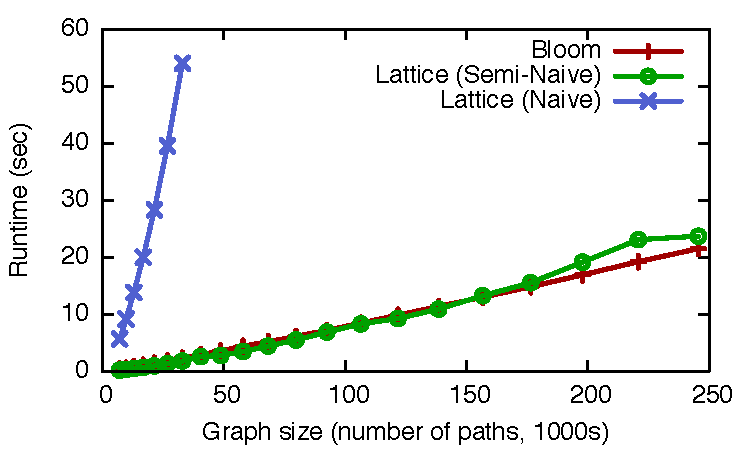
\includegraphics[width=\linewidth]{fig/sn_perf}
\caption{Performance of three different methods for computing the
  transitive closure of a graph.}
\label{fig:tc-perf-graph}
\end{figure}

To validate the effectiveness of semi-naive evaluation for \lang programs, we
wrote two versions of a program to compute the transitive closure of a directed
acyclic graph. One version was written in Bloom and used Bloom collections. The
other version was written in \lang using morphisms over the \texttt{lset}
lattice. For the \lang version, we ran the program both with and without
semi-naive evaluation enabled. As input, we generated synthetic graphs of
various sizes---in a graph with $n$ nodes, each node had $O(\log_2 n)$ outgoing
edges. We ran the experiment using a 2.13 Ghz Intel Core 2 Duo processor and 4GB
of RAM, running Mac OS X 10.7.4 and Ruby 1.9.3-p194. We ran each program variant
five times on each graph and report the mean elapsed wall-clock time.

Figure~\ref{fig:tc-perf-graph} shows how the runtime of each program varied with
the size of the graph. Note that we only report results for the naive \lang
strategy on small input sizes because this variant ran very slowly as the graph
size increased. The poor performance of naive evaluation is not surprising:
after deriving all paths of length $n$, naive evaluation will then rederive all
those paths at every subsequent round of the fixpoint computation. In contrast,
after computing length $n$ paths, a semi-naive strategy will only generate
length $n+1$ paths in the next round. Bloom and semi-naive \lang achieve similar
results. We instrumented Bud to count the number of derivations made by the
Bloom and semi-naive lattice variants---as expected, both programs made a
similar number of derivations. These results suggest that our implementation of
semi-naive evaluation for \lang is effective and performs comparably with
a traditional implementation of semi-naive evaluation for sets.

For large inputs, Bloom began to outperform the semi-naive lattice variant. We
suspect this is because the lattice implementation copies more data than Bloom
does for this benchmark. Lattice elements are immutable, so the \texttt{lset}
merge function allocates a new object to hold the result of the merge. In
contrast, Bloom collections are modified in-place. We plan to improve the
lattice code to avoid copies when it can determine that in-place updates are
safe.  \jmh{Argue that we already implemented this special-case reasoning for sets in Bloom?}

\subsection{Modifying Bud}
We were able to extend Bud to support \lang with relatively minor changes. Bud
initially had about 7200 lines of Ruby source code (LOC). The core lattice
features (the \texttt{Bud::Lattice} base class and the mapping from identifiers
to lattice elements) required about 300 LOC. Modifying Bud's fixpoint logic to
include lattices required only 10 LOC, while the program rewriting required to
enable semi-naive evaluation required 100 LOC. Modifying Bud's collection
classes to support merging of embedded lattice values required adding or
modifying about 125 LOC. The built-in lattice classes constituted an additional
300 LOC. In total, adding support for \lang required less than 900 lines of
added or modified code, and took about two person-months of engineering time.% This
% experience suggests that support for lattices can be added to an existing
% Datalog engine in a relatively straightforward manner.

\section{Case Study: Key-Value Store}
\label{sec:kvs}
The next two sections contain case studies that show how \lang can be used to
build practical distributed programs. Both case studies are monotonic programs:
that is, both programs consist of monotone functions applied to lattices. This
ensures that the values computed by the programs ``grow'' over time---these
examples show the various kinds of forward progress that can be encoded using
\lang.

In the first case study, we show that a distributed key-value store can be
\emph{composed} via a series of monotone mappings between simple lattices. This
demonstrates that \lang's built-in lattices are useful and results in a very
concise implementation. Moreover, it gives us confidence in the correctness of
our implementation, because much of the program's complexity is handled by the
behavior of the built-in lattices, which are likely to be correct.
\paa{not sure what to suggest, but this last clause seems underconfident 
(and slightly run-on).
perhaps we just want to say that we assert them to be correct, or that it's easy
to prove/convince ourselves that they are correct due to their simplicity, etc}

\subsection{Basic Architecture}
\begin{figure}[t]
\begin{scriptsize}
\begin{lstlisting}
module KvsProtocol
  state do
    channel :kvput, [:reqid, :@addr] => [:key, :val,
                                         :client_addr]
    channel :kvput_resp, [:reqid] => [:@addr, :replica_addr]
    channel :kvget, [:reqid, :@addr] => [:key, :client_addr]
    channel :kvget_resp, [:reqid] => [:@addr, :val,
                                      :replica_addr]
  end
end
\end{lstlisting}
\end{scriptsize}
\caption{Key-value store interface.}
\label{fig:kvs-interface}
\end{figure}

\begin{figure}[t]
\begin{scriptsize}
\begin{lstlisting}
class KvsReplica
  include Bud
  include KvsProtocol

  state { lmap :kv_store } (*\label{line:kvs-map-ddl}*)

  bloom do
    kv_store   <= kvput {|c| {c.key => c.val}} (*\label{line:kvs-put-merge}*)
    kvput_resp <~ kvput {|c| [c.reqid, c.client_addr, ip_port]}
    kvget_resp <~ kvget {|c| [c.reqid, c.client_addr,
                              kv_store.at(c.key), ip_port]}
  end
end
\end{lstlisting}
\end{scriptsize}
\caption{KVS replica implementation in \lang.}
\label{fig:kvs-replica}
\end{figure}

A key-value store (KVS) provides a lookup service that allows client
applications to retrieve the \emph{value} associated with a given \emph{key}. In
a typical KVS, key-value pairs are replicated on multiple server replicas for
redundancy and the keyspace is partitioned in some fashion to improve aggregate
storage and throughput. \emph{Eventual consistency} is a common correctness
criterion: after all client updates have reached all storage nodes, all the
replicas of a key-value pair will converge to the same final
state~\cite{Terry1995,vogels}.

Figure~\ref{fig:kvs-interface} shows a simple KVS interface in \lang. Client
applications submit \emph{get(key)} and \emph{put(key, val)} operations by
inserting into the \texttt{kvget} and \texttt{kvput} channels, respectively;
server replicas return responses via the \texttt{kvget\_resp} and
\texttt{kvput\_resp} channels.

Figure~\ref{fig:kvs-replica} contains the \lang code for a KVS server
replica. An \texttt{lmap} lattice is used to maintain the mapping between keys
and values (line~\ref{line:kvs-map-ddl}). Since the values in an \texttt{lmap}
lattice must themselves be lattice elements, for now we assume that clients only
want to store and retrieve lattice values; we discuss how to support arbitrary
values in Section~\ref{sec:kvs-versions}. To handle a \emph{put(key, val)}
request, a new \emph{key} $\to$ \emph{val} map is created and merged into
\texttt{kv\_store} (line~\ref{line:kvs-put-merge}). If \texttt{kv\_store}
already contains a value for the given key, the two values will be merged
together using the value lattice's merge function (see
Section~\ref{sec:lattice-built-ins} for details). Note that we use the \lang
features described in Section~\ref{sec:bloom-interop} to enable interoperability
between code that accesses traditional Bloom collections (e.g., channels) and
lattices (e.g., the \texttt{kv\_store} lattice).  Note that \texttt{ip\_port} is
a built-in function that returns the IP address and port number of the current
Bud instance.

The state of two replicas can be synchronized by simply exchanging their
\texttt{kv\_store} maps; the \texttt{lmap} merge function will automatically
resolve all conflicting updates made to the same key. This property allows
considerable flexibility in how replicas can choose to propagate updates.
% TODO: (1) finish repl discussion (composition, replication strat) (2) partitioning

\subsection{Object Versioning}
\label{sec:kvs-versions}
\begin{figure}[t]
\centering
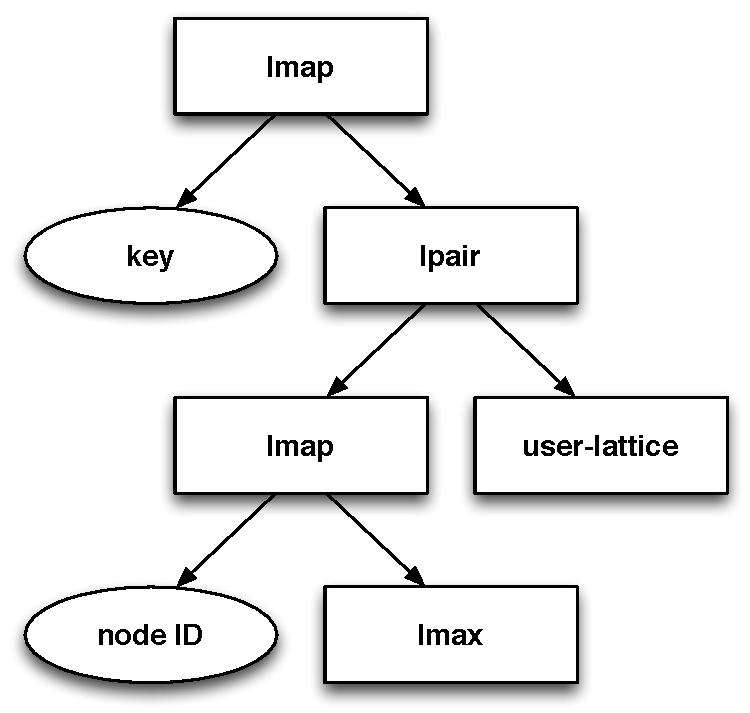
\includegraphics[width=0.8\linewidth]{fig/kvs-vc-lattice.pdf}
\caption{Lattice structure of a KVS with object versioning. Rectangles are
  lattices and ovals are atomic values.}
\label{fig:kvs-vc-lattices}
\end{figure}

The basic KVS design is sufficient for applications that want to store
monotonically increasing values, such as session logs or increasing counters. To
allow storage of values that change in arbitrary ways, we now consider how to
support \emph{object versions}. This is a classic technique for recognizing
mutual inconsistency between members of a distributed system~\cite{Parker1983};
our design is similar to that used by Dynamo~\cite{DeCandia2007}.

Each replica associates keys with
$\langle\textit{vector-clock},\textit{value}\rangle$ pairs. The vector clock
(VC) captures the causal relationship between different versions of a
record~\cite{Fidge1988,DeCandia2007}. Clients get and put
$\langle\textit{vector-clock},\textit{value}\rangle$ pairs. When a client
updates a value it has previously read, the client increments its own position
in the VC and includes the updated vector clock $V_U$ with its \emph{put}
operation. Upon receiving an update, the server compares $V_U$ with the VC of
the server's version of the record ($V_S$). If $V_U > V_S$, the server replaces
the stored record with the client's update. If $V_S > V_U$, the update is
ignored (this situation might arise due to duplication and reordering of
messages by the network). If $V_U$ and $V_S$ are incomparable, the two versions
are concurrent, so a client-supplied reconciliation function is used to resolve
the conflict.

From a \lang perspective, each replica still stores a monotonically increasing
value---the only difference is that in this scheme, the \emph{version} stored by
a replica increases over time, rather than the associated value. Hence, we now
consider how to support vector clocks and version-value pairs using \lang.

\subsubsection{Vector Clocks}
\nrc{Ugh, TODO.}
Vector clocks are a well-known mechanism for recording the causal relationships
between events~\cite{Fidge1988}. A vector clock is a map from node identifiers
to logical clocks. Each event $e$ is associated with a vector clock $V_e$; if
$V_e < V_{e'}$, $e$ causally precedes $e'$.

In \lang, a vector clock can be represented as an \texttt{lmap} that maps node
identifiers to \texttt{lmax} values. \texttt{lmax} is appropriate, since the
logical clock value associated with a given node will only increase over
time. The merge function provided by \texttt{lmap} achieves the desired
semantics.

\subsubsection{Version-Value Pairs}
We now turn to representing $\langle\textit{vector-clock},\textit{value}\rangle$
in \lang. To do this, we define a new lattice \texttt{lpair} that ``wraps'' two
lattice elements; we use \emph{fst} and \emph{snd} to refer to the first and
second elements of an \texttt{lpair}, respectively. The discussion above
suggests a natural least upper bound for \texttt{lpair}:
\begin{displaymath}
  A \sqcup B = \left\{
    \begin{array}{l l}
      A & \textrm{if } A.\textit{fst} > B.\textit{fst} \\
      B & \textrm{if } A.\textit{fst} < B.\textit{fst} \\
      \langle A.\textit{fst} \sqcup B.\textit{fst}, A.\textit{snd} \sqcup B.\textit{snd}\rangle & \textrm{otherwise} \\
    \end{array} \right. 
\end{displaymath}
This implements the desired semantics: given two candidate values for a key, the
candidate with the strictly greater version number should be preferred. When the
two versions are incomparable, a new \texttt{lpair} should be formed by merging
both elements of the input pairs with one another. In the case of the KVS,
\emph{fst} is a vector clock, while \emph{snd} is the user's data; applying the
least upper bound for the \emph{snd} lattice corresponds to invoking a
user-defined merge function.\footnote{If the user stores a value that does not
  have a merge function, similar systems typically provide a default merge
  function that collects conflicting updates for eventual manual resolution by
  the user. Such a strategy could easily be implemented with \lang.}

Note that while the \emph{fst} of a given \texttt{lpair} increases over time (as
new versions are received), the \emph{snd} may not (a newer version might
contain a ``smaller'' \emph{snd}). Again, this is the desired behavior.

\subsubsection{Discussion}
Figure~\ref{fig:kvs-vc-lattices} shows the lattices used in the KVS with object
versioning. Surprisingly, adding support for object versioning did not require
\emph{any} changes to the KVS replica code! Instead, clients simply store
\texttt{lpair} values containing a vector clock as the first element and
increment their position in the vector clock when submitting updates. The KVS
replica merges these \texttt{lpair} values into an \texttt{lmap} as usual; the
merge function of \texttt{lpair} handles conflict resolution in the appropriate
manner. Moreover, by composing the KVS from a collection of simple lattices, we
found it easy to reason about the behavior of the system. For example,
convincing ourselves that the KVS replicas will eventually converge only
required checking that the individual \texttt{lmap}, \texttt{lmax}, and
\texttt{lpair} lattices satisfy the lattice properties, rather than analyzing
the behavior of the system as a whole.

Our design compares favorably to traditional implementations of object
versioning and vector clocks. For example, the implementation of vector clocks
in Voldemort (a popular key-value store) requires 216 lines of Java source code,
not including whitespace or comments~\cite{voldemort-vector-clock}. In \lang,
vector clocks follow directly from the composition of the \texttt{lmap} and
\texttt{lmax} lattices; the entire KVS requires only 53 lines of Ruby and \lang
code, including the client library. The \texttt{lpair} lattice required 30 lines
of Ruby but is completely generic, and would be suitable for inclusion as a
built-in lattice.

\subsection{Quorum Reads and Writes}
A common KVS feature is the ability to submit reads and writes to a configurable
number of nodes. If a client reads from $R$ nodes and writes to $W$ nodes in a
KVS with $N$ replicas, the user can set $R + W > N$ to achieve behavior
equivalent to a quorum replication system~\cite{Gifford1979}, or use smaller
values of $R$ and $W$ if eventual consistency is sufficient. This scheme allows
users to vary $R$ and $W$ on a per-operation basis, depending on their
consistency and durability requirements.

To support this feature, we can use the \lang quorum voting pattern first
introduced in Figure~\ref{fig:lattice-quorum}. After sending a write to $W$
systems, the KVS client accumulates \texttt{kvput\_response} messages into an
\texttt{lset}. Testing for quorum can be done in a monotonic fashion by mapping
the \texttt{lset} to an \texttt{lmax} (using the \texttt{size} method), and then
performing a threshold test using \texttt{gt\_eq} on \texttt{lmax}. As expected,
this is monotonic: once quorum has been reached, it will never be retracted.

Quorum reads work in a similar fashion, except that the client must also merge
together the $R$ different versions of the record it receives (so-called ``read
repair''~\cite{DeCandia2007}). This follows naturally from the discussion in
Section~\ref{sec:kvs-versions}: the client can simply take the least upper bound
of all the values it receives, which produces the expected behavior. The client
can optionally write the merged value back to the KVS; note that the
\texttt{lpair} merge method also updates the record's vector clock
appropriately.

\section{Case Study: Shopping Carts}
\label{sec:carts}

\begin{figure}[t]
\centering
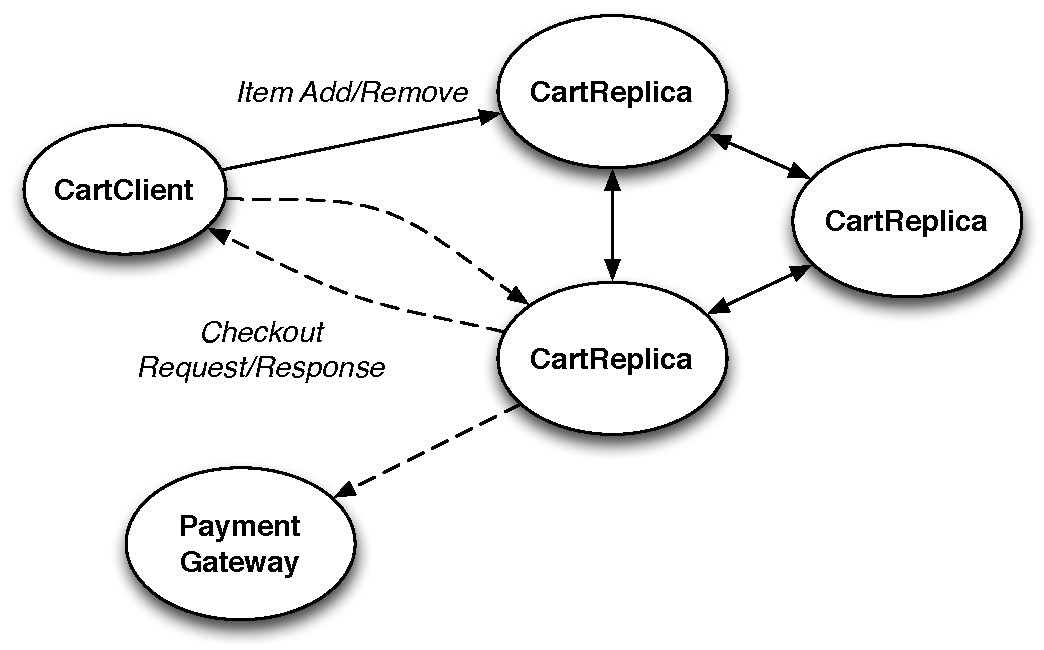
\includegraphics[width=\linewidth]{fig/cart_arch.pdf}
\caption{Shopping cart system architecture.}
\label{fig:cart-system-arch}
\end{figure}

In the previous section, we showed how a complete, consistent distributed
program can be composed via monotonic mappings between simple lattice types. In
this section, we describe how \lang overcomes the ``type dilemma'' of Bloom. In
prior work, we introduced a case study in Bloom that required the use of
coordination because of apparently-nonmonotonic grouping and
aggregation~\cite{Alvaro2011}; by using custom lattice types, we enable the
\lang CALM analysis to verify that our revised design is eventually consistent
without need for coordination.

%  we focus on the way that \lang enables us to overcome the ``type
% dilemma'' of Bloom, by demonstrating the use of custom lattice types.  Our
% previous implementation of this case study in Bloom called for coordination due
% to apparently-nonmonotonic grouping and aggregation~\cite{Alvaro2011}; by using
% custom lattice types in the implementation here, we enable the \lang CALM
% analysis to verify eventual consistency without any coordination.

% This feature of \lang allows developers to
% encode notions of ``forward progress'' for data types that are suited to the application.
% 
% ; as we will
% see, this allows more programs to be shown to be monotonic. Presenting monotonic
% implementations in \lang is equivalent to showing that the use of aggregation in
% these protocols is ``safe'' and produces consistent results without needing
% additional coordination.

In this case study, we consider a simple e-commerce system in which clients
interact with a shopping cart service by adding and removing items over the
course of a shopping session (Figure~\ref{fig:cart-system-arch}). The cart
service is replicated to improve fault tolerance; client requests can be routed
to any server replica. Eventually, a client submits a ``checkout'' operation, at
which point the cumulative effect of their shopping session should be summarized
and returned to the client. In a practical system, the result of the checkout
operation might be presented to the client for confirmation or submitted to a
payment processor to complete the e-commerce transaction. This case study is
based on the cart system from Alvaro et al.~\cite{Alvaro2011}, which was in turn
inspired by the discussion of replicated shopping carts in the Dynamo
paper~\cite{DeCandia2007}.

% Alvaro et al.\ discuss two different designs: a ``disorderly'' version in which
% the cart state is represented as a set of operations (allowing monotonic
% accumulation of adds and removes) and a ``destructive'' version in which the
% cart state is managed by a key-value store, which requires a non-monotonic
% update on each cart action.

\subsection{Monotonic Checkout}
\label{sec:monotone-checkout}

\begin{figure}[t]
\begin{scriptsize}
\begin{lstlisting}
module CartProtocol
  state do
    channel :action_msg,
      [:@server, :session, :op_id] => [:item, :cnt]
    channel :checkout_msg,
      [:@server, :session, :op_id] => [:lbound, :addr]
    channel :response_msg,
      [:@client, :session] => [:summary]
  end
end

module MonotoneReplica
  include CartProtocol

  state { lmap :sessions }

  bloom do
    sessions <= action_msg do |m|
      c = LCart.new({m.op_id => [ACTION, m.item, m.cnt]}) (*\label{line:cart-action-op}*)
      { m.session => c }
    end
    sessions <= checkout_msg do |m|
      c = LCart.new({m.op_id => [CHECKOUT, m.lbound, m.addr]}) (*\label{line:cart-checkout-op}*)
      { m.session => c }
    end

    response_msg <~ sessions do |session, cart| (*\label{line:cart-response-start}*)
      cart.is_complete.when_true {
        [cart.checkout_addr, session, cart.summary]
      }
    end (*\label{line:cart-response-end}*)
  end
end
\end{lstlisting}
\end{scriptsize}
\caption{Cart server replica in \lang that supports a monotonic
  (coordination-free) checkout operation.}
\label{fig:monotone-cart}
\end{figure}

% For both the ``disorderly'' and ``destructive'' designs, 
Alvaro et al.\ argue that processing a checkout request is non-monotonic because
it requires aggregating over an asynchronously computed data set---in general,
coordination might be required to ensure that all inputs have been received
before the checkout response can be returned to the client. However, observe
that the client knows exactly which add and remove operations should be
reflected in the result of the checkout. If that information can be propagated
to the cart service, any server replica can decide if it has enough information
to safely process the checkout operation without needing additional
coordination. This design is monotonic: once a checkout response is produced, it
will never change or be retracted. Our goal is to translate this design into a
monotonic \lang program.

% This can be done by assigning IDs to each message sent by the client. Each
% client has a session ID; within a session, operation IDs are assigned in
% increasing numeric order without gaps. Hence, if the client sends a ``lower
% bound'' message ID along with the checkout message, any replica of the cart
% service can independently ensure that it only produces a response message once
% it has received all the operations in the ID range indicated by the client. This
% essentially requires a threshold test over the operation IDs received by a given
% replica, which can easily be implemented using \lang.

Figure~\ref{fig:monotone-cart} contains the server code for this design (we omit
the client code for the sake of brevity). Communication with the client occurs
via the channels declared in the \texttt{CartProtocol} module. Each server
replica stores an \texttt{lmap} lattice that associates session IDs with
\texttt{lcart} lattice elements. An \texttt{lcart} is a custom lattice that
represents the state of a single shopping cart. An \texttt{lcart} contains a set
of client operations. Each operation has a unique ID; operation IDs are assigned
by the client in increasing numeric order without gaps. An \texttt{lcart}
contains two kinds of operations, \emph{actions} and \emph{checkouts}. An action
describes the addition or removal of an item from the cart. An \texttt{lcart}
contains at most one checkout operation---the checkout specifies the smallest
operation ID that must be reflected in the result of the checkout, along with
the address where the checkout response should be sent. The \texttt{lcart} merge
function takes the union of the operations in both input carts (operation IDs
ensure idempotence). In Figure~\ref{fig:monotone-cart},
lines~\ref{line:cart-action-op} and \ref{line:cart-checkout-op} construct
\texttt{lcart} elements that contain a single action or checkout operation,
respectively. These singleton carts are then merged with the previous
\texttt{lcart} associated with the client's session, if any.

An \texttt{lcart} is \emph{complete} if it contains a checkout operation as well
as all the actions in the ID range identified by the checkout. Hence, testing
whether an \texttt{lcart} is complete is a monotone function: it is similar to
testing whether an accumulating set has crossed a threshold. Hence, if any
server replica determines that it has a complete cart, it can send a response to
the client without risking inconsistency.\footnote{Without coordination, the
  client might receive multiple responses but they will all reflect the same
  cart contents.} Because this program contains only monotonic operations,
CALM analysis can verify that this design is consistent without requiring
additional coordination.

Note that the statement that produces a response to the client
(lines~\ref{line:cart-response-start}--\ref{line:cart-response-end}) is
contingent on having a complete cart. The monotone \texttt{summary} method
returns a summary of the actions in the cart---an exception is raised if
\texttt{summary} is called on an incomplete cart. Similarly, attempting to
construct an ``illegal'' \texttt{lcart} instance (e.g., an \texttt{lcart} that
contains multiple checkout operations or actions that are outside the ID range
specified by the checkout) also produces an exception, since this likely
indicates a logic error in the program.
% Implementing the \texttt{lcart} lattice required 58 lines of Ruby using the
% lattice API described in Section~\ref{sec:lattice-api}.

\subsection{Discussion}
This design is feasible because a single client has complete knowledge of the
shopping actions in its associated session. Hence, there is no need for
additional distributed coordination---the server replicas accumulate knowledge
but do not contribute new information themselves. If multiple clients could
operate on a single shopping cart, some form of coordination between the clients
would be needed to ensure a consistent checkout result.

Note that the threshold test for completeness is a crucial part of this
design. Until a cart is complete, its content changes in a ``non-monotonic''
fashion as items are added and removed. However, those non-monotonic changes are
hidden inside the \texttt{lcart} type and are not directly visible to
clients. Clients can only observe the cart's state once the cart is complete; at
that point, the cart state is immutable and hence will not change in a
non-monotonic fashion. \lang enables \texttt{lcart} to expose a limited ``safe''
interface and to hide transient non-monotonic changes from direct visibility.

% Note that because each replica determines when the cart is ``complete''
% independently, multiple response messages may be produced. However, they will
% all be consistent, because ...

% \subsection{Performance Study}
% \begin{itemize}
% \item
%   goal: demonstrate that removing coordination from a distributed protocol can
%   significantly reduce its running time
% \item
%   benchmark: destructive cart w/ coordination on each action vs.\ destructive
%   cart in \lang without coordination, disorderly cart with coordination on
%   checkout vs.\ disorderly cart with monotonic checkout
% \end{itemize}

\section{Related Work}
\label{sec:relwork}
The shopping cart case study in Section~\ref{sec:case} was motivated by the
Amazon Dynamo paper~\cite{dynamo}, as well as the related discussion by Helland
and Campbell~\cite{quicksand}. Systems with loose consistency requirements have
been explored in depth by both the systems and database management communities
(e.g.,~\cite{sagas,leases,dangers,bayou}); we do not attempt to provide
an exhaustive survey here.

The Bloom language is inspired by earlier work that attempts to integrate
databases and programming languages.  This includes early research such as
Gem~\cite{gem} and more recent object-relational mapping layers like Ruby on
Rails.  Unlike these efforts, Bloom is targeted at the development of both
distributed infrastructure and distributed applications, so it does not make any
assumptions about the presence of a database system ``underneath it.''  Given
our prototype implementation in Ruby, it is tempting to integrate Bud with
Rails; we have left this for future work.

Our work on Bloom bears a resemblance to the Reactor
language~\cite{reactors}. Both languages target distributed programming and are
grounded in Datalog. Moreover, both languages combine declarative rules and
state into a single program construct. While Bloom uses a syntax inspired by
object-oriented languages, Reactor takes a more explicitly agent-oriented
approach. Reactor also includes synchronous coupling between agents as a
primitive; we have opted to only include asynchronous communication as a
language primitive and to provide synchronous coordination between nodes as a
library. Another significant different is that, like many rule-based languages,
Reactor includes some imperative constructs (e.g., \ldots), whereas rules in
Bloom are purely declarative.

Another recent language related to our work is Coherence~\cite{coherence}, which
also embraces ``disorderly'' programming. Unlike Bloom, Coherence is not
designed for distributed computing and is not based on logic programming.

There is a long history of attempts to design programming languages more
suitable to parallel and distributed systems; for example, Argus~\cite{argus}
and Linda~\cite{linda}.  Again, we do not hope to survey that literature here.
More pragmatically, Erlang is an oft-cited choice for distributed programming in
recent years.  Erlang's features and design style encourage the use of
asynchronous lightweight ``actors.''  As mentioned previously, we did a simple
Bloom prototype DSL in Erlang (which we cannot help but call ``Bloomerlang''),
and there is a natural correspondence between Bloom-style distributed rules and
Erlang actors.  However there is no requirement for Erlang programs to be
written in the disorderly style of Bloom. It is not obvious that typical Erlang
programs are significantly more amenable to a useful points-of-order analysis
than programs written in any other functional language.  For example, ordered
lists are basic constructs in functional languages, and without program
annotation or deeper analysis than we need to do in Bloom, any code that
modifies lists would need be marked as a point of order, much like our
destructive shopping cart.  We believe that Bloom's ``disorderly by default''
style encourages more disorderly programming; we know that its roots in database
theory bore fruit in terms of our analysis.  While we would be happy to see the
analysis ``ported'' to currently popular distributed programming environments,
it may be that design patterns using Bloom-esque disorderly programming are the
natural way to achieve this.

\section{Discussion and Future Work}
\label{sec:discussion}

\lang simplifies the design of loosely consistent distributed systems by
enabling \emph{composability}. Rather than reasoning about the consistency of an
entire application, the programmer can instead ensure that individual lattices
satisfy \emph{local} correctness properties (e.g., commutativity, associativity,
and idempotence). The CALM analysis then verifies that when these modules are
composed to form an application, the complete program satisfies the desired
consistency properties.

Nevertheless, designing a correct lattice can still be difficult. To address
this, we plan to develop tools to give programmers more confidence in the
correctness of lattice implementations. For example, we plan to build a test
data generation framework that can efficiently cover the space of possible
inputs to lattice merge functions. We also plan to explore a restricted DSL for
writing lattice methods, which would make formal verification of correctness an
easier task.

Each lattice includes $\bot$, a distinguished ``smallest element.'' A natural
extension is to consider whether any lattices would support $\top$, a ``greatest
element.'' In fact, such a value is already supported by \texttt{lbool} ($\top =
\mathtt{true}$), in addition to the \texttt{lcart} lattice discussed in
Section~\ref{sec:monotone-checkout}. $\top$ behaves differently than other
lattice elements: because it is immutable, any function can safely be applied to
it (whether monotone or not), without risking inconsistency. Since the merge
function for $\top$ will always yield $\top$, this might allow a more efficient
representation (e.g., in a complete \texttt{lcart}, we need only store the
``summarized'' cart state, not the log of client operations). We are
investigating how our program analysis could be enhanced to provide special
support for lattices with $\top$ values.

As discussed in Section~\ref{sec:causal}, \lang is still useful even when
confluence is not an appropriate correctness criteria. Nevertheless, a global
program analysis for classes of non-confluent programs would be very useful. For
example, we can show that each node's local vector clock increases over
time. However, we would like to show something stronger for programs that use
causal delivery: whenever a new message is delivered, it should contain ``new''
information. If not, the newly delivered message ``happens before'' the state of
the recipient, which implies that causality has been violated (assuming
at-most-once delivery). A program analysis to prove that this situation never
occurs would require reasoning about intermediate states of the program, rather
than considering only final states (as in confluence).

% By allowing a more general notion of monotonicity, \lang significantly increases
% the number of programs that can be shown to be confluent. However, many
% distributed protocols are not intended to be confluent---rather, they exhibit
% \emph{controlled non-determinism}, in which timing conditions affect the choice
% of one among several acceptable outcomes. Vector clocks and causal delivery are
% both examples of this kind of behavior. Although \lang is still useful---the
% local correctness properties of lattices help programmers to reason about the
% behavior of individual program values---we are also investigating\ldots

% Support a notion of sealing?

\section{Conclusion}
\label{sec:conclusion}
And thus, we conclude.
%\section{Case Study: Causal Delivery}
\label{sec:causal}

Vector clocks are a classical mechanism for recording the causal relationships
between events in a distributed system~\cite{Fidge1988,Mattern1989}. In this
section, we first show how vector clocks can be implemented in a monotonic
fashion using \lang. We then use \lang to implement a classical algorithm for
point-to-point causal message delivery~\cite{Schiper1989}. The implementation of
both protocols in \lang is concise and readable---this suggests that \lang is
suitable for common distributed programming tasks. Perhaps more significantly,
both protocols are monotonic. This agrees with our intuition that these
protocols make ``progress'' over time, and hence gives us more confidence in the
correctness of our designs.

% Concede that confluence is not an appropriate correctness criteria

\subsection{Vector clocks}
\begin{figure}[t]
\begin{scriptsize}
\begin{lstlisting}
module VectorClock
  state do
    lmap :my_vc
    lmap :next_vc
    interface input, :in_msg, [:addr, :payload] => [:clock]
    interface input, :out_msg, [:addr, :payload]
    interface output, :out_msg_vc, [:addr, :payload] => [:!clock] (*\label{line:ddl-lattice-merge}*)
  end

  bootstrap do
    my_vc <= {ip_port => Bud::MaxLattice.new(0)}
  end

  bloom do
    next_vc <= my_vc
    next_vc <= out_msg { {ip_port => my_vc.at(ip_port) + 1} } (*\label{line:vc-out-increment}*)
    next_vc <= in_msg  { {ip_port => my_vc.at(ip_port) + 1} } (*\label{line:vc-in-increment}*)
    next_vc <= in_msg  {|m| m.clock} (*\label{line:vc-in-merge}*)
    my_vc <+ next_vc

    out_msg_vc <= out_msg {|m| [m.addr, m.payload, next_vc]} (*\label{line:vc-out-stamp}*)
  end
end
\end{lstlisting}
\end{scriptsize}
\caption{Vector clocks in \lang.}
\label{fig:vector-clock-src}
\end{figure}

A \emph{vector clock} is an array containing a logical clock for each node in
the distributed system. Each node keeps a local vector clock that it updates
when it sends and receives messages; the node's vector clock reflects how
up-to-date its local knowledge is with respect to the other nodes in the
system. Vector clocks can be used to assign a partial order over the events in
the system that agrees with the causal relationship between events.

Each node $n$ initializes its vector clock to $\{n \rightarrow 0\}$. A node
updates its vector clock $v$ by following three rules when sending and receiving
events:
\begin{compactenum}
\item
  Before sending a message, $n$ increments $v[n]$ and includes $v$ in the
  outgoing message.
\item
  Upon receipt of a message, $n$ increments $v[n]$.
\item
  Upon receipt of a message, $n$ merges the vector clock in the message with its
  own vector clock by taking the element-wise max of the logical clock values.
\end{compactenum}
Figure~\ref{fig:vector-clock-src} contains a complete implementation of vector
clocks in \lang. A vector clock is represented as a map lattice that associates
node IDs with \texttt{lmax} values. Each \texttt{lmax} represents a single
logical clock---naturally, a clock can only increase over time.
\texttt{ip\_port} returns the IP address and port number of the current \lang
instance, which is used as a node ID. Incoming messages appear in the
\texttt{in\_msg} collection. Messages that are intended to be sent begin as
tuples in \texttt{out\_msg}; once a message has been stamped with the local
node's vector clock, it appears in \texttt{out\_msg\_vc}.

The key logic appears in lines \ref{line:vc-out-increment},
\ref{line:vc-in-increment}, and \ref{line:vc-in-merge}: these three statements
are a direct translation of the three rules for updating a vector clock given
above. Line~\ref{line:vc-out-stamp} stamps outgoing messages with the updated
vector clock value.  Note that if multiple outgoing messages are sent in the
same \lang timestep, they will contain the same embedded vector clock (and
\texttt{my\_vc} will only be incremented once). This is reasonable, since those
messages are concurrent.

Figure~\ref{fig:vector-clock-src} is both concise and readable, and requires
only six \lang statements. This compares favorably with implementations of
vector clocks in traditional programming languages. For example, the
\texttt{VectorClock} class included with the Voldemort key-value store consists
of 216 lines of Java source code, not including whitespace or
comments~\cite{voldemort-vector-clock}.

Note that Figure~\ref{fig:vector-clock-src} is a monotonic program. Hence, its
statements can be executed in any order. The ``lattice embedding'' feature
described in Section~\ref{sec:lattice-embedding} ensures that the
\texttt{out\_msg\_vc} tuple contains a single vector clock that reflects all the
messages received in the current timestep. The monotonicity of the vector clock
program reflects our intuition that a node's vector clock increases over
time. Vector clocks can also be implemented in Bloom but they require the use of
non-monotonic operators (e.g., incrementing a node's clock requires
non-monotonic state update using $\verb|<+|$ and $\verb|<-|$, and merging the
clock values in inbound messages requires a \texttt{max} aggregate).

\subsection{Causal delivery}
\begin{figure}[t]
\begin{scriptsize}
\begin{lstlisting}
module CausalDelivery
  include VectorClock (*\label{line:causal-d-import}*)

  state do
    channel :chn, [:@dst, :payload] => [:clock, :ord_buf]
    table :recv_buf, chn.schema
    lmap :ord_buf
  end

  bloom :outbound_msg do
    chn <~ out_msg {|m| [m.addr, m.payload, next_vc, ord_buf]} (*\label{line:out-msg-embed}*)
    ord_buf <+ out_msg {|m| {m.addr => next_vc} } (*\label{line:ord-buf-out-msg}*)
  end

  bloom :inbound_msg do
    recv_buf <= chn
    in_msg <= recv_buf do |m| (*\label{line:deliver-msg-start}*)
      m.ord_buf.at(ip_port).lt_eq(my_vc).when_true { (*\label{line:deliver-msg-lt-eq}*)
        [m.addr, m.payload, m.clock]
      }
    end (*\label{line:deliver-msg-end}*)
    ord_buf <+ in_msg {|m| m.ord_buf} (*\label{line:ord-buf-in-msg}*)
  end
end
\end{lstlisting}
\end{scriptsize}
\caption{Point-to-point causal delivery in \lang. Note that \texttt{in\_msg} and
\texttt{out\_msg} are defined by the \texttt{VectorClock} module.}
\label{fig:causal-delivery-src}
\end{figure}

Next, we use \lang to build a more complex distributed protocol that makes use
of vector clocks. A \emph{causal delivery} protocol ensures that messages are
delivered in an order that is consistent with the ``happens before'' relation
between events~\cite{Lamport1978}. Avoiding causal anomolies is a common
building block for distributed protocols.

Figure~\ref{fig:causal-delivery-src} contains a \lang program that implements a
classical algorithm for point-to-point (unicast) causal delivery proposed by
Schiper et al.~\cite{Schiper1989}. Note the Ruby \texttt{import} statement on
line~\ref{line:causal-d-import}, which loads the \lang state declarations and
statements from the \texttt{VectorClock} module.

In the Schiper et al.\ protocol, each node records its knowledge about the state
of the vector clocks at every other node. In
Figure~\ref{fig:causal-delivery-src}, this knowledge is represented as
\texttt{ord\_buf} an \texttt{lmap} that associates node IDs with vector
clocks. A node's \texttt{ord\_buf} is updated when messages are sent or
delivered (lines~\ref{line:ord-buf-out-msg} and \ref{line:ord-buf-in-msg},
respectively). A node also embeds both its vector clock and \texttt{ord\_buf} in
outgoing messages (line~\ref{line:out-msg-embed}). Finally, the protocol ensures
that a node will delay delivering a message $m$ until it can be sure that it
will never receive a message that causally predeces $m$. This is done by
comparing the knowledge the sender had about the recipient's vector clock with
the recipient's current vector clock; once the recipient's vector clock passes
the sender's knowledge, the message can be safely delivered
(lines~\ref{line:deliver-msg-start}--\ref{line:deliver-msg-end}, respectively).

Note that checking whether a message has been delivered requires testing whether
one vector clock (in the \texttt{ord\_buf} embedded in the message) is smaller
than the node's vector clock (line~\ref{line:deliver-msg-lt-eq}). In general,
this is not monotonic because either vector clock might subsequently
increase. In this case, the message's vector clock is immutable (because it is
embedded as a column of a collection that does not allow ``lattice merges''), so
the predicate can be determined to be monotonic.


%\section{Acknowledgments}
Ras Bod\'{\i}k and Tyson Condie were intimately involved in discussions
surrounding the development of \lang.  We are also indebted to Mark Utting and
Erik Meijer for conversation and inspiration from their Starlog and LINQ
experiences respectively, and to Phil Bernstein for suggestions on future work.
Thanks to Jesse Trutna and Kuang Chen for comments on the paper. This work was
supported by NSF grants 0803690, 0722077 and 0713661, Air Force Office of
Scientific Research award 22178970-41070-F, the Natural Sciences and
Engineering Research Council of Canada, and gifts from Yahoo Research, IBM
Research and Microsoft Research.


\balance
\bibliographystyle{abbrv}
\bibliography{socc}

% \newpage
% \begin{appendix}
% \section{Proof of Lemma 1}
\begin{proof}
%First, we prove an isomorphism between stable models, and finite prefixes of stable models.  Scan a stable model of a program timestamp by timestamp.  
We first present an algorithm for computing ultimate models, and argue that the algorithm computes exactly the ultimate models of the \lang program.  We then argue this algorithm can be run on our operational formalism, and show how operational traces correspond with prefixes of stable models.

Any \lang program without asynchronous rules is a $\text{Datalog}_{1S}$ program, and the algorithm given in~\cite{tdd} computes its ultimate model in polynomial space\footnote{The class of {\em multi-seperable}~\cite{tdd-poly} \lang programs, which comprises all \lang programs $P$ with guarded asynchrony and persisted EDB, and their coordinations $\textsc{Coord}(P)$, can be executed in polynomial time in the size of the input.} in the size of the input.  The algorithm evalutes the program for $2^G + e$ consecutive timesteps, where $G$ is the number of instantiations of the non-temporal attributes of the program rules using all combinations of constants in the Herbrand Universe, and $e$ is the maximum timestamp of any EDB fact.  At each step, the algorithm updates information on observed periodicities of facts.  When the algorithm terminates, any fact with a periodicity of 1 is regarded as part of the ultimate model.

For asynchronous rules, the natural distributed analog of the above algorithm simultaneously executes one instance for each node \dedalus{n}, using values of $G$ and $e$ computed from $E_{\text{\dedalus{{\scriptsize n}}}}$.  Each instance has its own local clock, which corresponds to the timestamp attribute in the model-theoretic semantics.  Nodes communicate over channels with arbitrary delay and message re-ordering.  When a remote node \dedalus{m} derives a fact at \dedalus{n}, it encloses its local clock value, \dedalus{t}; \dedalus{n} must consider this fact at his local time \dedalus{t} or later, in the style of Lamport Clocks.  Note that this behavior is equivalent to the model-theoretic semantics of remote asynchronous rules: remote deductions are visible at the destination at a time later than the body temporal attribute at the source.  Further, note that Lamport Clocks only introduce the constraint that if message $a$ ``happens before'' $b$, in other words $a$ directly or transitively causes $b$ to be sent, then $T(a) < T(b)$.  If $a$ and $b$ are concurrent, there is some execution where $T(a) \geq T(b)$.

When \dedalus{n} processes a received message, the number of constants available to \dedalus{n} may increase, and thus the node's $G$ may increase to $G'$.  Furthermore, the node may need to execute over this new fact for $2^{G'}$ additional timesteps.  If only finitely many messages are sent, this algorithm terminates, and requires polynomial space.  In the case that infinitely many messages are sent, we only need to process each message $2^{G'}$ times: the maximum period of any fact is $2^{G'}$, as every incoming fact needs to have a chance (in some execution) to join with any deduction (with which it is ``concurrent'') at any time during its period.  Keeping track of the number of times we have seen each fact also requires polynomial space.  When the algorithm is done running for $2^{G'}$ steps, it pauses, waiting for new network input that it has not seen enough times.  If all nodes are paused and no outstanding messages exist, then the collection of all period 1 facts at all instances of the algorithm comprises an ultimate model.

We claim that the algorithm can generate every ultimate model---every message has the opportunity to join with another concurrent message or its transitive consequents at any point during their period, and has the opportunity to join with a causally related message during the range of times allowed by the model-theoretic constraint (identical to the Lamport Clock condition used in the algorithm).  Furthermore, the set of all facts, and their local timestamps, comprises a prefix of a stable model.

Note that we can execute this algorithm straightforwardly on our operational formalism.  Evaluating a single timestamp of a \lang program corresponds to the evaluation of a Datalog program, which is a polynomial time computation, and the Turing Machines can also maintain the necessary state about periods and message counts.
%2) Intuitively, the operational model is based on n Turing Machines, one per value of node(), which independently step sequentially through time and communicate via channels with
%non-deterministic delay.  At each timestep t they run a datalog fixpoint computation that evaluates P on ``projection(E_n, t)'' (notation needed); this takes polynomial
%time~\cite{immerman}.  At the end of this fixpoint there are three sets of relevant facts: local, synchronous facts that have timestep t+1 and become part of ``projection(E_n,
%t)'', local asynchronous facts whose timestep is chosen non-deterministically to be greater than t and become part of later timesteps, and remote asynchronous facts.  The
%timestamps in this third class of facts are chosen non-deterministically ``at the receiver'' to model delay, in a way that observes traditional causality
%restrictions~\cite{lamportclocks}.
%3) Any \lang program without  async rules is a Datalog_{1S} program, and the above intuition is captured by the algorithm given in~\cite{}, computing an ultimate model in
%polynomial space in the size of the input.  In the presence of asynchronous rules, this formalize needs to be expanded to account for the asynchronous advancement of time through
%\dedalus{successor} at each node.  The PSPACE guarantees of~\cite{} are not shown to hold for such programs, but in Appendix Foo we show that the following Lemma holds for all
%\lang programs under this model
\end{proof}

\section{Proof of Lemma 2}
\begin{proof}
We begin by assuming that \dedalus{node} contains the identifiers of each of the $n$ nodes.  Since the atemporal fragment of \lang is FO[LFP], we can represent a polynomial-time bounded Turing Machine using only atemporal rules in \lang~\cite{immerman-ptime}.  In addition to normal operations, the Turing Machine can place items into a queue---\cite{dedalus} shows how to model queues in \lang---or send messages to other nodes---modeled by an asynchronous communication rule with \dedalus{queue} in the head.  A node persists the contents of the tape across time if the queue is empty, using a rule like \dedalus{tape(\dbar{X})@next <- tape(\dbar{X}), !queue(\dbar{\_});}.  If the queue is non-empty, the computation skips a timestamp (leaving \dedalus{tape} empty), and then atomically copies the contents of \dedalus{queue} to \dedalus{tape}.  The ultimate model of this program is exactly the final contents of the tape on every node if the computation halts.  Otherwise, the program's ultimate model is empty: \dedalus{tape} facts only exist every other timestamp, and for any Turing Machine predicate \dedalus{r} we can create \dedalus{r'}, and create a mutual recursive cycle to ensure neither \dedalus{r} nor \dedalus{r'} contains facts at every timestamp:

\begin{Dedalus}
r(\dbar{X})@next <- r'(\dbar{X});
r'(\dbar{X})@next <- r(\dbar{X});
\end{Dedalus}

We can play a somewhat similar trick for \dedalus{queue} by having local messages alternate between going into \dedalus{queue} and \dedalus{queue'}.  Thus, no local queue message will be part of the ultimate model.  Remote messages will still go into \dedalus{queue}: this still leaves the case that the exact same message repeatedly arrives at a node at every timestamp forever, by chance.  We can dispense of this case by assuming the channels interconnecting the Turing Machines forbid it.
\end{proof}

\section{Proof of Lemma 3}
\begin{proof}
Our proof proceeds via construction of a two counter machine in \lang, inspired by the construction in~\cite{undecidable-datalog}.

We represent the state of a two counter machine using the \linebreak \dedalus{cnfg(T,S,C1,C2)} relation, where \dedalus{T} represents ``time'' (note this is not the same as the \lang temporal attribute), \dedalus{S} is the state, and \dedalus{C1} and \dedalus{C2} are the values of the two counters.  In order to support our two instructions, $inc$ and $dec$, we would like to make use of the \dedalus{successor} relation.  However, \lang conventions forbid the use of this infinite relation outside of the timestamp attribute.  Thus, we posit the \dedalus{fin\_succ(X,Y)} EDB relation, which is meant to represent a finite prefix of the \dedalus{successor} relation.  Since it is EDB, its contents may be arbitrary.  If \dedalus{fin\_succ} is malformed, then the machine's execution may be incorrect.  In particular, our model of the machine may accept an input, whereas the actual machine would not have accepted that input.  We illustrate how to constrain the contents of \dedalus{fin\_succ} below:

\begin{Dedalus}
malformed() <- fin_succ(_,0);
malformed() <- fin_succ(X,Y), fin_succ(X,Z), Y != Z;
malformed() <- fin_succ(Y,X), fin_succ(Z,X), Y != Z;
malformed() <- fin_succ(X,Y), X >= Y;
\end{Dedalus}

For a given EDB, the two counter machine either halts in the accepting state or halts in a non-accepting state.  It cannot run forever since the EDB (in particular, the \dedalus{fin\_succ} relation) is finite.

We construct a \lang program that nondeterministically decides to either run the machine on the input provided (and for the length of \dedalus{fin\_succ} provided, or declare that the machine will never accept without running it.  If the machine ever accepts some input, this induce two different ultimate models---one generated by a trace where we run the machine and it accepts, and one generated by a trace where we decide to not run the machine, and thus we implicitly reject.  We describe the program below. 

Initially, we nondeterministically decide whether to run the machine or not by sending two messages (0 and 1) to a remote node (\dedalus{decider}).  If both message arrive simultaneously, then the decider responds to run the machine.  Otherwise, the decider responds to declare failure:

%\jmh{should we use a hashmark for constants?  I would say no.}
\begin{Dedalus}
//send two messages to the decider
message(#D, 0)@async <- decider(D);
message(#D, 1)@async <- decider(D);

//decider responds to computer
run_machine(#computer)@async <- message(0),
                                message(1);
declare_failure(#computer)@async <- message(0),
                                    !message(1);
declare_failure(#computer)@async <- !message(0),
                                    message(1);
\end{Dedalus}

Each mapping in the transition function is expressed by a \lang rule with \dedalus{!malformed()} and \dedalus{!declare\_failure()} in its body.  For example, the rule $\delta(3, > =) = (7, inc, dec)$ would be represented as:

\begin{Dedalus}
cnfg(S,7,D1,D2) <- cnfg(T,3,C1,C2), C1 > 0, C2 == 0,
                   fin_suc(T, S), fin_succ(C1, D1),
                   fin_succ(D2, C2), !malformed(),
                   !declare_failure();
\end{Dedalus}

We declare success or failure as follows:

\begin{Dedalus}
reject() <- !accept();
accept() <- cnfg(20,_,_); //20 is the accepting state
accept()@next <- accept();
\end{Dedalus}

If we choose to declare failure, or the machine halts in a non-accepting state---whether it is due to incompleteness or malformedness of \dedalus{fin\_succ}, or actual halting---then the ultimate model will contain \dedalus{reject}.  If the machine halts in an accepting state, then the ultimate model will contain \dedalus{accept}.  Thus, if we can decide confluence of this program, then we can decide whether there is any input for which an arbitrary two-counter machine halts.
\end{proof}

% \end{appendix}

\end{document}
